\documentclass[11pt]{article}
\usepackage{natbib}
\usepackage{url}
\usepackage[utf8]{inputenc} % Codificación
\usepackage{amsmath}
\usepackage{graphicx}
\graphicspath{{images/}} % Carpeta en la cual se van a buscar las imagenes
\usepackage{subfigure}	% Permite la Inclusión de subfiguras
%\usepackage{parskip} % Borrar identación de parrafos.
\setlength{\parskip}{3mm} % Longitud del espaciado entre parrafos
\usepackage[hidelinks]{hyperref} % Referencias (links)
\usepackage{fancyhdr}
\usepackage{vmargin}
\setpapersize{A4} % Formato del papel - A4
\setmarginsrb{3 cm}{2.5 cm}{3 cm}{2.5 cm}{1 cm}{1.5 cm}{1 cm}{1.5 cm} % Margenes
\usepackage{paralist} % Permite un mayor control sobre las listas
\usepackage{textcomp,marvosym,pifont} % Generación de símbolos especiales
\usepackage[usenames,dvipsnames,svgnames,x11names,table]{xcolor}

%%%%%%%%%%%%%%%%%%%%%%%%%%%%%%%%%%%%%%%%%%%%%%%%%%%%%%%%%%%%%%%%%%%%%%%%%%%%%%%%%%%%%%%%%
% Complemento para insertar código en la memoria:
% A partir de 'Listados de código cómodos y resultones con listings' de David Villa
% http://crysol.org/es/node/909

\usepackage{color}
\definecolor{gray97}{gray}{.97}
\definecolor{gray75}{gray}{.75}
\definecolor{gray45}{gray}{.45}

\usepackage{listings}
\lstset{ frame=Ltb,
	framerule=0pt,
	aboveskip=0.5cm,
	framextopmargin=3pt,
	framexbottommargin=3pt,
	framexleftmargin=0.4cm,
	framesep=0pt,
	rulesep=.4pt,
	backgroundcolor=\color{gray97},
	rulesepcolor=\color{black},
	texcl=true,
	%
	stringstyle=\ttfamily,
	showstringspaces = false,
	basicstyle=\small\ttfamily,
	commentstyle=\color{gray45},
	keywordstyle=\bfseries,
	%
	numbers=left,
	numbersep=13pt,
	numberstyle=\tiny,
	numberfirstline = false,
	breaklines=true,
}

% minimizar fragmentado de listados
\lstnewenvironment{listing}[1][]
{\lstset{#1}\pagebreak[0]}{\pagebreak[0]}

\lstdefinestyle{consola}
{basicstyle=\scriptsize\bf\tiny,
	backgroundcolor=\color{gray75},
}

\lstdefinestyle{C}
{language=C,
}
%%%%%%%%%%%%%%%%%%%%%%%%%%%%%%%%%%%%%%%%%%%%%%%%%%%%%%%%%%%%%%%%%%%%%%%%%%%%%%%%%%%%%%%%%

\usepackage{float} % Permite usar H en las figuras, de manera que se coloquen en la posición exacta en la que están en el código.


% Añade un comando para crear indicaciones de pulsación de teclas
\usepackage{tikz} % Paquete especializado en gráficos
\usetikzlibrary{shadows} % Necesario para poder crear nuevo comando de indicación de pulsación de tecla.
\newcommand*\tecla[1]{%   
	\tikz[baseline=(key.base)]
	\node[%
	draw,
	fill=white,
	drop shadow={shadow xshift=0.25ex,shadow yshift=-0.25ex,fill=black,opacity=0.75},
	rectangle,
	rounded corners=2pt,
	inner sep=1pt,
	line width=0.5pt,
	font=\scriptsize\sffamily
	](key) {#1\strut}
	;
}

\newif\ifspanish % Condicional que permite seleccionar el lenguage.
\spanishtrue


%%%%%%%%%%%%%%%%%%%%%%%%%%%%%%%%%%%%%%%%%%%%%%%%%%%%%%%%%%%%%%%%%%%%%%%%%%%%%%%%%%%%%%%%%
%%%%%%%%%					Principales variables del documento					%%%%%%%%%

\title{Práctica 4. Gestión de prioridad de tráfico en IP.}							% Titulo
\author{Alberto Salas Seguín y Marcos López Sobrino.}							% Autor
\date{\today}											% Fecha
\newcommand{\subject}{Planificación e Integración de Sistemas y Servicios.}						% Asignatura
\newcommand{\course}{4º Grado en Ingeniería Informática.}		% Curso

%\spanishfalse	% Descomentar esta línea si el trabajo está en inglés

%%%%%%%%%%%%%%%%%%%%%%%%%%%%%%%%%%%%%%%%%%%%%%%%%%%%%%%%%%%%%%%%%%%%%%%%%%%%%%%%%%%%%%%%%

\ifspanish
	\usepackage[spanish]{babel} % Paquete de español
	\newcommand{\dateText}{Fecha:}
	\renewcommand{\lstlistingname}{Listado} % Renombrar listados para que aparezcan en español.
	% Algoritmos
	\usepackage[ruled,vlined,spanish]{algorithm2e} % Permite pseudocódigos. NECESARIO INSTALAR texlive-science (sudo apt-get install texlive-science)
\else
	\usepackage[english]{babel} % Paquete de inglés
	\newcommand{\dateText}{Date:}
	% Algoritmos
	\usepackage[ruled,vlined,english]{algorithm2e}
\fi

\makeatletter
\let\thetitle\@title
\let\theauthor\@author
\let\thedate\@date
\makeatother

\pagestyle{fancy}
\fancyhf{}
\rhead{\theauthor}
\lhead{Práctica 4.}
\cfoot{\thepage}

\begin{document}
\begin{titlepage}
	\centering
    
\includegraphics[scale = 0.25]{esilogo.png}\\[1.0 cm]	% Logo de la universidad
    \textsc{\LARGE Universidad de Castilla-La Mancha}\\[0.5 cm]	% Nombre de la universidad
    \textsc{\LARGE Escuela Superior de Informática}\\[2.0 cm]
	\textsc{\Large \textbf{\subject}}\\[0.5 cm]				% Asignatura
	\textsc{\large \course}\\[0.5 cm]						% Curso
	\rule{\linewidth}{0.2 mm} \\[0.4 cm]
	{ \huge \bfseries \thetitle}\\
	\rule{\linewidth}{0.2 mm} \\[1.5 cm]
	
	\begin{minipage}{0.4\textwidth}
		\begin{flushleft} \large
			\emph{Autor:}\\
			\textbf{\theauthor}
			\end{flushleft}
			\end{minipage}~
			\begin{minipage}{0.4\textwidth}
			\begin{flushright} \large
			\emph{\dateText} \\
			\thedate
		\end{flushright}
	\end{minipage}\\[1.5 cm]
 
	\vfill
	
\end{titlepage}

\section{Entorno de trabajo.}
El entorno de trabajo utilizado han sido 3 máquinas virtuales gestionadas mediante Vagrant, con la imagen \textbf{\textit{ubuntu/trusty64}}. Una de ellas actúa como cliente, otra como servidor y otra como router entre ambas. A continuación, explicamos la configuración de las redes, de las máquinas, y los paquetes instalados.
\begin{figure}[hbtp]
\centering
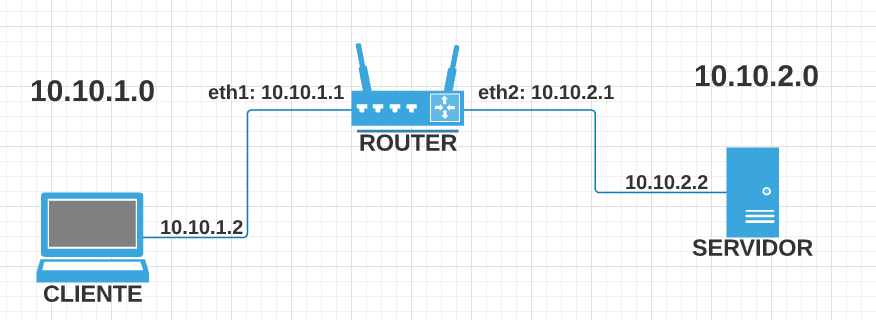
\includegraphics[scale=0.5]{top.png}
\caption{Topología de la red.}
\end{figure}

\subsection{Cliente y servidor.} 
Como vemos en la figura anterior, la red del cliente, que corresponde a la interfaz \textbf{eth1} del router, tiene como IP \textbf{10.10.1.0}; mientras que la red del servidor, que corresponde a la interfaz \textbf{eth2} del router, tiene como IP \textbf{10.10.2.0}. \\ \\
Para el correcto funcionamiento de las comunicaciones, hay que indicarle a la máquina cuál es la ruta por defecto, para ello, se ejecutan los siguientes comandos:

\begin{lstlisting}[style=C, numbers=none]
$ sudo ip route del default dev eth0
$ sudo ip route add default via <ip_router> dev eth1
\end{lstlisting}
donde \textit{ip\_router} sería la dirección IP de la interfaz del router dentro de la red correspondiente. \\ \\
\newpage
Los paquetes necesarios para el funcionamiento de la práctica en el caso del cliente y el servidor son:
\begin{itemize}
\item \textbf{iptables}
\item \textbf{iperf}
\item \textbf{sip-tester}
\end{itemize}

\subsection{Router.}
A la máquina del router se le ha instalado un entorno gráfico para poder usar cómodamente la herramienta \textbf{Wireshark}. Además, se le han asignado 2048 MB de RAM. Por otra parte, se ha configurado las interfaces de red con la dirección \textbf{.1} de la red correspondiente, tal y como vemos en la figura. Adicionalmente, para que la máquina actúe como router se debe activar el \textbf{IP forwarding}, para ello, en el playbook correspondiente del router se ha añadido una regla específica. \\ \\
Por último, en el router se han instalado los siguientes paquetes:
\begin{itemize}
\item Para la interfaz gráfica:
	\begin{itemize}
		\item \textbf{xorg}
		\item \textbf{gnome-core}
		\item \textbf{gnome-system-tools}
		\item \textbf{gnome-app-install}
	\end{itemize}
\item \textbf{wireshark}
\item \textbf{iptables}			
\end{itemize}

\subsection{Archivos de configuración e inicialización.}
Todo lo anterior se recoge en el archivo \textbf{\textit{Vagrantfile}} y los distintos \textbf{\textit{playbooks}}, que se pueden encontrar junto a este documento. Para poner en funcionamiento el entorno de trabajo, ejecutamos:
\begin{lstlisting}[style=C,numbers=none]
	vagrant up --provision
\end{lstlisting}

\section{Marcado de paquetes.}
\subsection{Configuración de iptables en router, cliente y server.}
Dado que tanto en la máquina del router como la del cliente, se van a introducir reglas de iptables para el correcto funcionamiento, para no perder estas reglas se va a utilizar \textbf{\textit{iptables-persistent}}, el modo para recuperar todas las reglas cada vez que se inicie la máquina es mediante una \textit{task} cuya función es cargar un archivo con todas las reglas necesarias en el directorio \textbf{\textit{/etc/iptables/rules.v4}}, este directorio se encuentra tanto en la máquina del router como en la máquina del cliente. La regla que hemos utilizado para copiar este archivo en el directorio mencionado es la siguiente:

\begin{lstlisting}[style=C,numbers=none]
- name: copy iptables
  copy:
    src: <archivo a copiar>
    dest: /etc/iptables/rules.v4
    owner: root
    group: root
    mode: 0644
  notify: "restore iptables"
\end{lstlisting}

Como vemos en el código anterior, en la última línea se hace mención a \textbf{\textit{notify}}, lo cual hace necesario la presencia de un manejador, de manera que cada vez que se invoque a la tarea \textbf{\textit{copy tables}}, se va a hacer el \textit{notify}, cuya función es hacer un \textbf{restore} del archivo \textbf{/etc/iptables/rules.v4} que hemos copiado. Esto lo podemos ver en el siguiente código:

\begin{lstlisting}[style=C,numbers=none]
handlers:
    - name: restore iptables
      shell: iptables-restore /etc/iptables/rules.v4
      listen: "restore iptables
\end{lstlisting}

\newpage
\subsection{Reglas iptables utilizadas en router, cliente y server.}
\begin{itemize}
\item \textbf{Router.}
	\begin{itemize}
	En el caso del router hemos utilizado las reglas iptables que vienen dadas en el enunciado de la práctica. Estas son:
\begin{lstlisting}[style=C,numbers=none]		
iptables -t filter -A INPUT -m dscp --dscp 14 -m limit --limit 5/s --limit-burst 5 -j ACCEPT

iptables -t filter -A INPUT -m dscp --dscp 14 -j DROP		
\end{lstlisting}
	Donde los parámetros --limit y --limit-burst significan lo siguiente.
	\item \textbf{limit.} El módulo limit se utiliza para restringir la tasa de coincidencias, por ejemplo, para suprimir los mensajes de registro. Sólo coincidirá con un número determinado de veces por segundo (por defecto 3 coincidencias por hora, con una ráfaga de 5). Se necesitan dos argumentos opcionales: 
		\begin{itemize}
			\item \textbf{-limit.} Seguido de un número y una unidad, especifica el número medio máximo de coincidencias que puede permitirse por segundo. Nos permite configurar el tiempo que tiene que pasar para que esta regla se cumpla entre dos paquetes.
			\item \textbf{--limit-burst.} Seguido de un número que indica la cantidad máxima de paquetes antes de que se active el límite anterior. \\
		\end{itemize}
	\end{itemize}
	
\item \textbf{Client.}
	Dado que vamos a marcar paquetes, la tabla que vamos a usar es \textbf{mangle}. Por un lado, el tráfico RTP lo vamos a marcar con \textbf{Expedited Forwarding}, el \textbf{DSCP} recomendado para Expedited Forwarding es \textbf{46 (101110)}. Por otro lado, el tráfico SIP lo vamos a marcar como \textbf{Assured Forwarding 11}, cuyo valor es 10. De modo que las reglas nos quedan de la siguiente manera:
\begin{lstlisting}[style=C,numbers=none]
iptables -t mangle -A OUTPUT -p udp --dport 5060 -j DSCP --set-dscp 10

iptables -t mangle -A OUTPUT -p udp --dport 10000:20000 -j DSCP --set-dscp 46

iptables -A OUTPUT -j DSCP --set-dscp 0
\end{lstlisting}
\begin{itemize}

\item La primera regla permite el tráfico udp saliente del cliente que tiene como puerto destino (dport) el puerto 5060, el cual es el puerto dedicado al protocolo SIP. Como hemos dicho antes, este tráfico se ha marcado con AF11 con el valor 10.

\item La segunda regla permite el tráfico udp saliente del cliente que tiene como destino el rango de puertos que corresponden al protocolo RTP (10000:20000) y dicho tráfico se ha marcado como Expedited Forwarding con el valor 46.
\end{itemize}

\item La tercera regla se utiliza para el marcado de paquetes Best Effort.

\item \textbf{Server.}
Las reglas son las mismas que en el cliente, %sólo con una diferencia, que en lugar de utilizar \textbf{--dport} (destination port), en el server se va a utilizar \textbf{--sport} (source port), lo demás, está configurado igual que en las reglas del cliente.
\begin{lstlisting}[style=C,numbers=none]
iptables -t mangle -A OUTPUT -p udp --sport 5060 -j DSCP --set-dscp 10

iptables -t mangle -A OUTPUT -p udp --sport 10000:20000 -j DSCP --set-dscp 46

iptables -A OUTPUT -j DSCP --set-dscp 0x00
\end{lstlisting}

\end{itemize}
\newpage

\section{Análisis del rendimiento.}
Para la realización de este apartado se va a utilizar la herramienta \textbf{iperf}. Lo primero que vamos a hacer es utilizar la herramienta para ver cual es el ancho de banda sin incluir las reglas iptables definidas en el apartado anterior. Para establecer la comunicación:
\begin{lstlisting}[style=C,numbers=none]
$ iperf -s 			// Máquina del server.
$ iperf -c 10.10.2.2 -i 2	// Máquina del router.
\end{lstlisting}

Tras realizar esta prueba, los resultados son los siguientes:

\begin{lstlisting}[style=C,numbers=none]
root@router:/home/vagrant# iperf -c 10.10.2.2 -i 2
------------------------------------------------------------
Client connecting to 10.10.2.2, TCP port 5001
TCP window size: 85.0 KByte (default)
------------------------------------------------------------
[  3] local 10.10.2.1 port 37999 connected with 10.10.2.2 port 5001
[ ID] Interval       Transfer     Bandwidth
[  3]  0.0- 2.0 sec   290 MBytes  1.22 Gbits/sec
[  3]  2.0- 4.0 sec   301 MBytes  1.26 Gbits/sec
[  3]  4.0- 6.0 sec   301 MBytes  1.26 Gbits/sec
[  3]  6.0- 8.0 sec   293 MBytes  1.23 Gbits/sec
[  3]  8.0-10.0 sec   293 MBytes  1.23 Gbits/sec
[  3]  0.0-10.0 sec  1.44 GBytes  1.24 Gbits/sec
\end{lstlisting}

Si ahora esta misma prueba la hacemos incluyendo las llamadas de \textbf{sipp}, el resultado es el siguiente:

\begin{lstlisting}[style=C,numbers=none]
root@router:/home/vagrant# iperf -c 10.10.2.2 -i 2
------------------------------------------------------------
Client connecting to 10.10.2.2, TCP port 5001
TCP window size: 85.0 KByte (default)
------------------------------------------------------------
[  3] local 10.10.2.1 port 38063 connected with 10.10.2.2 port 5001
[ ID] Interval       Transfer     Bandwidth
[  3]  0.0- 2.0 sec   230 MBytes   964 Mbits/sec
[  3]  2.0- 4.0 sec   251 MBytes  1.05 Gbits/sec
[  3]  4.0- 6.0 sec   234 MBytes   983 Mbits/sec
[  3]  6.0- 8.0 sec   241 MBytes  1.01 Gbits/sec
[  3]  8.0-10.0 sec   238 MBytes   999 Mbits/sec
[  3]  0.0-10.0 sec  1.17 GBytes  1.00 Gbits/sec
\end{lstlisting}

Vemos que ya el ancho de banda es más bajo que cuando únicamente se utilizaba iperf. Esta reducción es debido al tráfico generado por \textit{sipp}.

Llegados aquí, introducimos las reglas iptables para realizar las mismas pruebas anteriores.\\
Con las reglas iptables activadas y con iperf, el resultado es el siguiente:
\begin{lstlisting}[style=C,numbers=none]
Client connecting to 10.10.2.2, TCP port 5001
TCP window size: 85.0 KByte (default)
------------------------------------------------------------
[  3] local 10.10.2.1 port 53610 connected with 10.10.2.2 port 5001
[ ID] Interval       Transfer     Bandwidth
[  3]  0.0- 2.0 sec   269 MBytes  1.13 Gbits/sec
[  3]  2.0- 4.0 sec   276 MBytes  1.16 Gbits/sec
[  3]  4.0- 6.0 sec   285 MBytes  1.20 Gbits/sec
[  3]  6.0- 8.0 sec   290 MBytes  1.22 Gbits/sec
[  3]  8.0-10.0 sec   296 MBytes  1.24 Gbits/sec
[  3]  0.0-10.0 sec  1.38 GBytes  1.19 Gbits/sec
\end{lstlisting}
Observamos de nuevo, que el ancho de banda es menor que en el primer listado de código, donde no se utilizaba ni \textit{iptables} ni \textit{sipp}. Con esto deducimos que el marcado de los paquetes está funcionando bien. \\

La última prueba es utilizando las reglas \textit{iptables} y \textit{sipp}, tras ejecutar dicha prueba el resultado es el siguiente:
\begin{lstlisting}[style=C,numbers=none]
root@router:/home/vagrant# iperf -c 10.10.2.2 -i 2
------------------------------------------------------------
Client connecting to 10.10.2.2, TCP port 5001
TCP window size: 85.0 KByte (default)
------------------------------------------------------------
[  3] local 10.10.2.1 port 53698 connected with 10.10.2.2 port 5001
[ ID] Interval       Transfer     Bandwidth
[  3]  0.0- 2.0 sec   239 MBytes  1.00 Gbits/sec
[  3]  2.0- 4.0 sec   241 MBytes  1.01 Gbits/sec
[  3]  4.0- 6.0 sec   251 MBytes  1.05 Gbits/sec
[  3]  6.0- 8.0 sec   262 MBytes  1.10 Gbits/sec
[  3]  8.0-10.0 sec   250 MBytes  1.05 Gbits/sec
[  3]  0.0-10.0 sec  1.21 GBytes  1.04 Gbits/sec
\end{lstlisting}

De nuevo, se ha reducido el ancho de banda. Se están produciendo descartes de paquetes marcados como Best Effort, mientras que los paquetes RTP y SIP tienen el ancho de banda necesario para sus comunicaciones.
\section{Bibliografía}

\begin{itemize}
	\item Configuración reglas Iptables.

	\url{https://netfilter.org/documentation/HOWTO/packet-filtering-HOWTO-7.html#ss7.3}\\ \\
	\url{https://www.cisco.com/c/en/us/support/docs/quality-of-service-qos/qos-packet-marking/10103-dscpvalues.html}\\ \\
	\url{https://community.rti.com/kb/how-set-dscp-flag-your-system}
	
	\item Acerca de sipp.
	
	\url{http://sipp.sourceforge.net/doc/reference.html}
\end{itemize}

\end{document}